% Smart Room Temperature Monitor -- CMPE 286 project report (IEEE conference format)
%
% Build:  cd docs/report && latexmk -pdf report.tex
% (or upload this folder plus ../data-flow.png, ../web-dashboard.png and
%  ../grafana-dashboard-simulated.png to Overleaf).
%
% Text in red (\fillin{...}) must be completed by the team before submission:
% names, hardware measurements that need the physical board, and the AI-use
% statement. Search for "fillin" to find them all.

\documentclass[conference]{IEEEtran}
\IEEEoverridecommandlockouts

\usepackage[T1]{fontenc}
\usepackage{amsmath}
\usepackage{newtxtext,newtxmath}
\usepackage{cite}
\usepackage{graphicx}
\usepackage{booktabs}
\usepackage{array}
\usepackage{xcolor}
\usepackage{url}
\usepackage[hidelinks]{hyperref}

\graphicspath{{../}}
\newcommand{\fillin}[1]{\textcolor{red}{[#1]}}
\newcommand{\code}[1]{\texttt{\small #1}}

\begin{document}

\title{Smart Room Temperature Monitor: An Edge-First IoT System with MQTT, Time-Series Storage, and Live Dashboards}

\author{
\IEEEauthorblockN{Nguyen Phuong Duy Lam}
\IEEEauthorblockA{\textit{Department of Computer Engineering} \\
\fillin{University} \\
\fillin{email}}
\and
\IEEEauthorblockN{Tri Ngo}
\IEEEauthorblockA{\textit{Department of Computer Engineering} \\
\fillin{University} \\
\fillin{email}}
\and
\IEEEauthorblockN{\fillin{Third member, or delete}}
\IEEEauthorblockA{\textit{Department of Computer Engineering} \\
\fillin{University} \\
\fillin{email}}
}

\maketitle

\begin{abstract}
Rooms that overheat are uncomfortable, reduce concentration, and can be dangerous for
vulnerable occupants or for equipment such as small server closets. This paper presents
the design, implementation, and evaluation of a low-cost Smart Room Temperature Monitor
built around a NodeMCU ESP8266 and a DHT11 sensor. The device reads temperature and
humidity every two seconds, computes the heat index, and raises a local alert on a
16$\times$2 LCD and a buzzer when a configurable threshold is reached, so it keeps
protecting the room even without a network. Readings are published over MQTT to a
containerized pipeline (Mosquitto, Telegraf, InfluxDB) and visualized in Grafana,
while the board also serves its own self-contained web dashboard with a 20-minute
history and remote controls. Online/offline state is reported with retained messages
and the MQTT Last Will. Because hardware was not always available, the firmware was
compiled and tested on a laptop against fake hardware libraries; 19 automated tests
and JSON contract checks found two real defects, including one that left the board
unresponsive 99\,\% of the time while the broker was unreachable (reduced to 11\,\%).
On the server side we measured a median MQTT broker hop of 1.7\,ms, a median
publish-to-storage latency of 4.6\,s, and offline detection within 0.01\,s after a
reset and 24\,s after a silent power loss.
\end{abstract}

\begin{IEEEkeywords}
Internet of Things, MQTT, ESP8266, environmental monitoring, InfluxDB, Grafana,
edge computing, embedded software testing
\end{IEEEkeywords}

% ---------------------------------------------------------------------------
\section{Introduction}

Indoor temperature has a direct effect on comfort, productivity, and health. Standards
such as ANSI/ASHRAE 55 describe the conditions under which most occupants find a space
thermally acceptable~\cite{ashrae55}, and the perceived temperature also depends on
humidity, which is why weather services report a heat index~\cite{rothfusz,steadman}.
Many rooms, however, have no monitoring at all: dormitories, rented apartments, labs,
and small equipment closets are often noticed to be too hot only after the fact.

Commercial smart thermostats address part of this problem but are tied to a vendor
cloud, usually control a single HVAC zone, and are not designed to be extended. Our
objective was to build an open, inexpensive monitor that (1)~measures temperature and
humidity continuously, (2)~warns people in the room immediately, (3)~lets them see
current and historical conditions from any phone or laptop, (4)~can be configured
remotely, and (5)~keeps working when parts of the network fail.

The main contributions of this project are:
\begin{itemize}
  \item An \emph{edge-first} design in which the alarm logic runs on the
        microcontroller, so alerts do not depend on Wi-Fi, the broker, or the server.
  \item Two complementary user interfaces: a self-contained web dashboard served by
        the ESP8266 itself, and a Grafana dashboard backed by a time-series database.
  \item An MQTT topic design with retained status, Last Will, and bidirectional
        command topics, connected to InfluxDB through Telegraf without custom server code.
  \item A host-based test harness that runs the unmodified firmware on a laptop against
        fake hardware, which found two defects before the hardware was available.
  \item Measurements of the latency and failure-detection behavior of the pipeline.
\end{itemize}

% ---------------------------------------------------------------------------
\section{Background and Related Work}

IoT systems are commonly described as layers of sensing, networking, and
application services~\cite{alfuqaha}. For the networking layer, several application
protocols are used: HTTP is universal but request/response only, CoAP targets very
constrained networks, and MQTT provides lightweight publish/subscribe messaging through
a broker~\cite{naik}. MQTT~\cite{mqtt311} fits our case well: the device sends small,
frequent messages, several consumers (database, dashboards, other tools) need the same
data, and commands must reach the device through the same connection. MQTT also
provides retained messages and a Last Will and Testament, which the broker publishes
when a client disconnects unexpectedly; we use both to track whether the device is
online. Eclipse Mosquitto is a widely used open-source MQTT broker~\cite{mosquitto}.

Time-series databases such as InfluxDB are optimized for timestamped measurements
and support windowed aggregation, which makes them a common choice for sensor
data~\cite{influxdb}. Telegraf is an agent that can subscribe to MQTT topics and write
the parsed messages into InfluxDB~\cite{telegraf}, and Grafana provides interactive
dashboards on top of it~\cite{grafana}. Hobby projects with the ESP8266 and DHT11 often
stop at an LCD or a single cloud service; our system combines local alerting, a local
web interface, and a full storage and visualization pipeline, and adds automated
testing of the firmware.

% ---------------------------------------------------------------------------
\section{System Design}

\subsection{Requirements}
The functional requirements were: sample temperature and humidity at least every few
seconds; show readings and alerts locally; alert when the temperature reaches a
threshold; allow the threshold to be changed and the buzzer to be muted remotely; store
history; and show both live and historical data. Non-functional requirements were low
cost, operation on a local network without internet access, tolerance to network and
sensor failures, and a design that other devices can join later.

\subsection{Architecture and Data Flow}
Fig.~\ref{fig:dataflow} shows the architecture. It has three zones. The \emph{edge
device} reads the sensor, decides whether to alert, drives the LCD and buzzer, keeps a
short history, and exposes data over HTTP and MQTT. The \emph{local Wi-Fi network}
carries two kinds of traffic: HTTP requests from browsers to the device, and MQTT
traffic between the device and the broker. The \emph{server}, a set of Docker
containers on a laptop, receives MQTT messages in Mosquitto; Telegraf subscribes to the
device topics and writes each message to InfluxDB, and Grafana queries InfluxDB.
Commands flow the other way: any MQTT client (or the device's own web page) can change
the threshold or mute the buzzer.

\begin{figure*}[t]
  \centering
  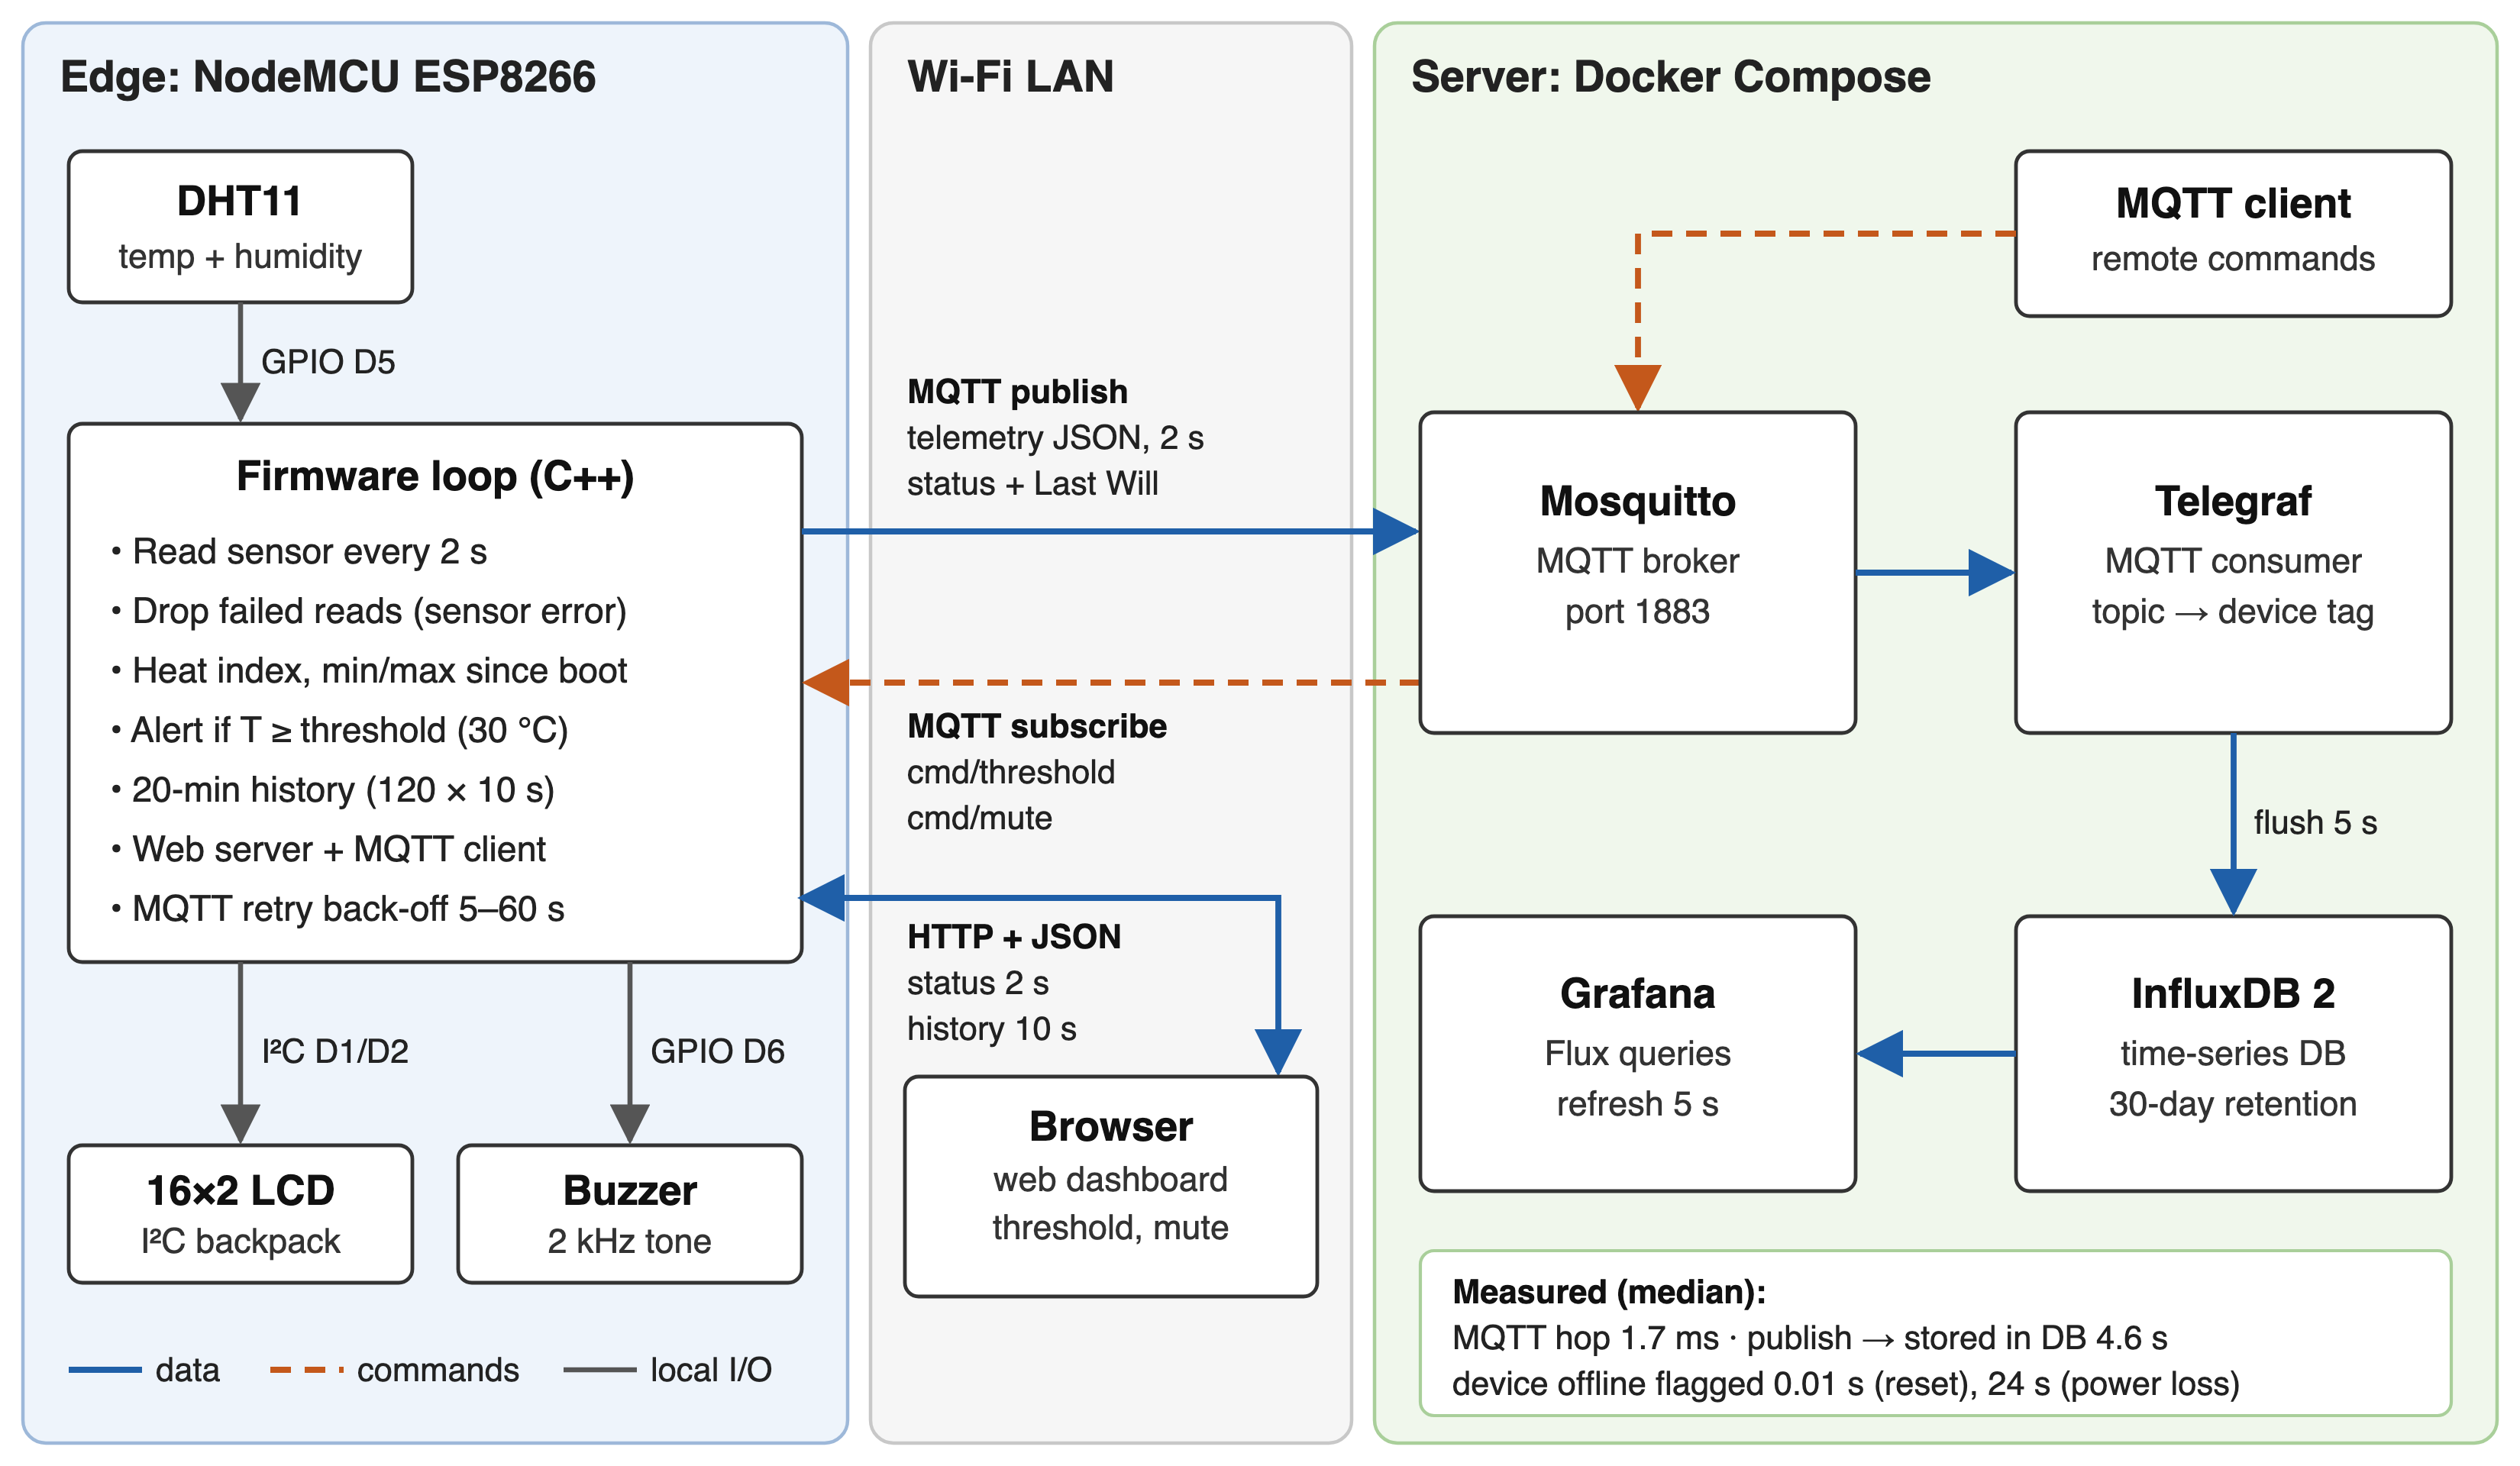
\includegraphics[width=\textwidth]{data-flow.png}
  \caption{Architecture and data flow. Solid blue arrows carry sensor data, dashed orange
  arrows carry commands, and gray arrows are local I/O on the board. The latency values were
  measured on the server side (Section~\ref{sec:eval}).}
  \label{fig:dataflow}
\end{figure*}

A key design decision is that the alarm is evaluated on the board. If the laptop is
off or Wi-Fi fails, the LCD and buzzer still work, and the web dashboard still works as
long as a browser can reach the board. The server adds history, analytics, and remote
access, but nothing safety-relevant depends on it.

\subsection{Hardware}
The device uses a NodeMCU board with an ESP8266 Wi-Fi microcontroller~\cite{esp8266},
a DHT11 temperature and humidity sensor, a 16$\times$2 character LCD with an I\textsuperscript{2}C
backpack, and a buzzer. Table~\ref{tab:wiring} lists the connections. The DHT11 is
specified for 0--50\,\textdegree C with $\pm$2\,\textdegree C accuracy and 20--90\,\% relative
humidity with $\pm$5\,\% accuracy, and should not be read more than once per
second~\cite{dht11}; a two-second sampling period respects this limit while still
reacting quickly to changes.

\begin{table}[t]
  \caption{Hardware Connections}
  \label{tab:wiring}
  \centering
  \begin{tabular}{@{}lll@{}}
    \toprule
    Component & Signal & NodeMCU pin \\
    \midrule
    DHT11 & Data & D5 (GPIO14) \\
    LCD backpack & SDA / SCL & D2 / D1 \\
    Buzzer & + & D6 (GPIO12) \\
    All & VCC / GND & 3V3 / GND \\
    \bottomrule
  \end{tabular}
\end{table}

\subsection{MQTT Topic and Data Model}
Every topic starts with \code{smartroom/} followed by the device identifier
(Table~\ref{tab:topics}), so adding a room only requires a new identifier. Telemetry is a flat JSON object
with numeric fields only (temperature, humidity, heat index, threshold, alert flag,
mute flag, sensor error count, Wi-Fi RSSI, and uptime). A typical message is 142\,bytes
of payload on a 25-byte topic, about 171\,bytes including the MQTT header; at one
message every two seconds this is 43\,200 messages and roughly 7.4\,MB per day per device.

Telemetry is published with QoS~0 because a lost reading is replaced two seconds later.
The status topic is retained and published with QoS~1, and the device registers
\code{offline} as its Last Will, so any new subscriber immediately learns the current
state and the broker announces an unexpected disconnect on the device's behalf.

\begin{table}[t]
  \caption{MQTT Topics Under \code{smartroom/<id>/}}
  \label{tab:topics}
  \centering
  \begin{tabular}{@{}l l >{\raggedright\arraybackslash}p{0.42\columnwidth}@{}}
    \toprule
    Topic & Direction & Payload \\
    \midrule
    \code{telemetry} & device $\rightarrow$ & JSON reading, every 2\,s \\
    \code{status} & device $\rightarrow$ & \code{online}/\code{offline}, retained, Last Will \\
    \code{cmd/threshold} & $\rightarrow$ device & threshold in \textdegree C \\
    \code{cmd/mute} & $\rightarrow$ device & \code{1} or \code{0} \\
    \bottomrule
  \end{tabular}
\end{table}

Telegraf parses the device identifier out of the topic and stores it as an InfluxDB
tag, so telemetry lands in the measurement \code{room\_climate} and status in
\code{device\_status}, both indexed by device. The bucket keeps 30 days of data.

% ---------------------------------------------------------------------------
\section{Implementation}

\subsection{Firmware}
The firmware is written in C++ with the Arduino core for the ESP8266, using the DHT,
LiquidCrystal\_I2C, and PubSubClient libraries. The main loop never blocks for long:
it services HTTP requests, maintains the MQTT connection, and uses \code{millis()}
timers to read the sensor every 2\,s and to store a history sample every 10\,s. A
failed read (the library returns NaN) sets a sensor-error state that is shown on the
LCD and the dashboards and counted, instead of being reported as a value.

The history for the web dashboard is a ring buffer of 120 samples of temperature and
humidity (20 minutes), which takes only 960\,bytes of RAM. The minimum and maximum
temperature since boot are also tracked. The threshold (valid range 0--60\,\textdegree C)
and the mute flag can be changed from the web page or over MQTT; both paths call the
same functions, which validate the value, update the LCD and buzzer immediately, and
publish a fresh telemetry message so Grafana shows the change without waiting for the
next reading.

When the broker cannot be reached, a TCP connection attempt can block for several
seconds. Reconnection attempts are therefore spaced with an exponential back-off from
5\,s up to 60\,s, measured from the end of the previous attempt (Section~\ref{sec:bugs}).

\subsection{On-Device Web Dashboard}
The ESP8266 serves a single-page dashboard (Fig.~\ref{fig:web}) stored in flash as a
22\,KB string, with no external libraries or fonts so that it works on a network
without internet access. The page polls a small JSON API: \code{GET /api/status} every
2\,s and \code{GET /api/history} every 10\,s; \code{POST /api/threshold} and
\code{POST /api/mute} change settings. It draws gauges and the 20-minute chart with
inline SVG, adapts to phone screens and dark mode, and shows a banner if the board
stops answering for more than 6\,s.

\begin{figure}[t]
  \centering
  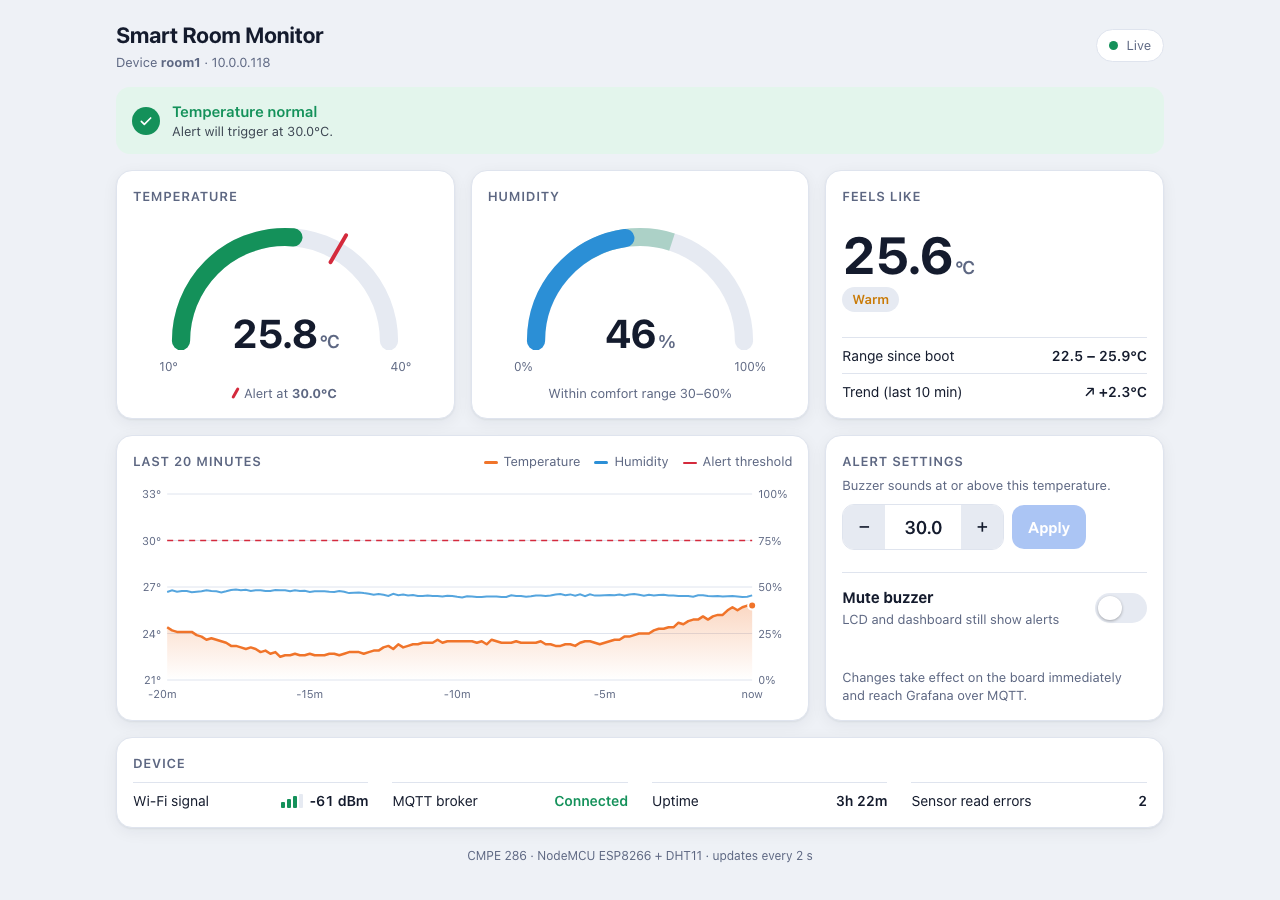
\includegraphics[width=\columnwidth]{web-dashboard.png}
  \caption{Web dashboard served by the ESP8266 (shown with the mock device used during
  development): gauges, heat index, 20-minute history, and alert settings.}
  \label{fig:web}
\end{figure}

\subsection{Server Pipeline and Grafana}
The server is defined in a Docker Compose file with pinned versions of Mosquitto
(2.0.20), InfluxDB (2.7.11), Telegraf (1.33.1), and Grafana (11.4.0), so the whole
stack starts with one command on any laptop. The InfluxDB data source and the dashboard
are provisioned automatically. The dashboard (Fig.~\ref{fig:grafana}) has three rows:
current values and device state, history with shaded comfort bands and an alert
timeline, and summary statistics for the selected time range, such as the share of time
spent in alert. Windows without data are kept empty, so periods when the device was
offline appear as gaps instead of misleading straight lines. The dashboard JSON is
generated by a Python script, which keeps the Flux queries readable and under version
control.

\begin{figure}[t]
  \centering
  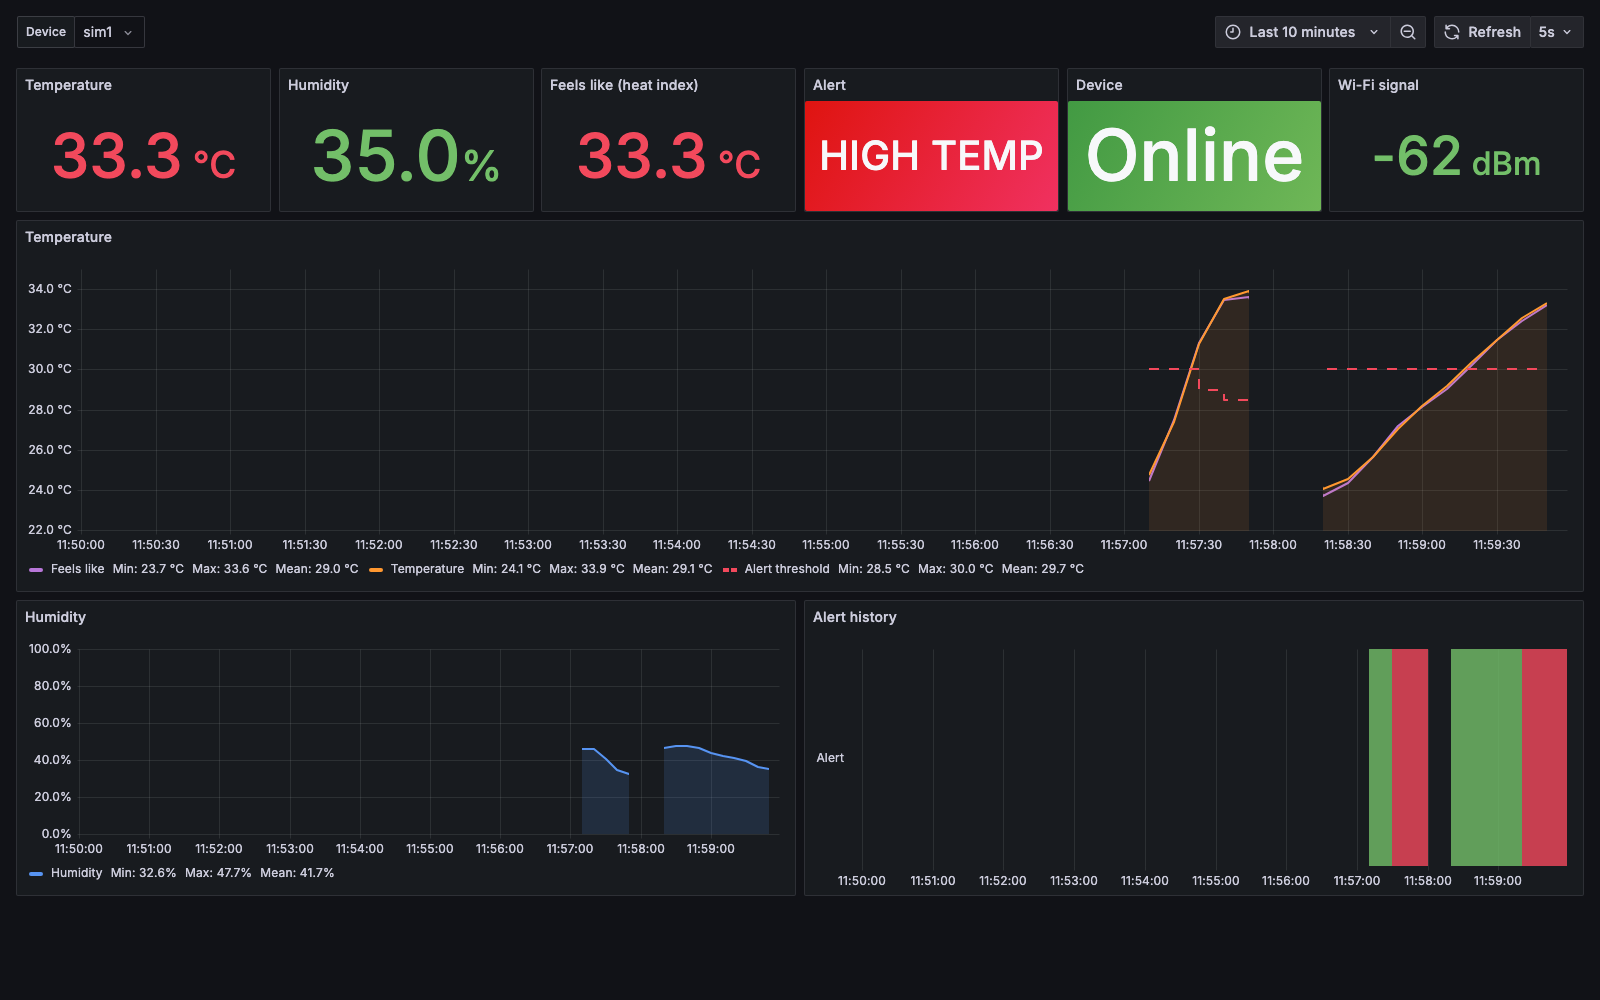
\includegraphics[width=\columnwidth]{grafana-dashboard-simulated.png}
  \caption{Grafana dashboard with data from the sensor simulator, including a simulated
  heat event that crosses the 30\,\textdegree C threshold.}
  \label{fig:grafana}
\end{figure}

\subsection{Development Tools}
A Python simulator publishes realistic telemetry (daily drift, noise, and an optional
heat ramp) with the same topics, payload, and Last Will as the board, and obeys the
command topics. It allowed the pipeline and dashboards to be developed before the
hardware was assembled and serves as a backup for the live demonstration.

% ---------------------------------------------------------------------------
\section{Testing and Evaluation}
\label{sec:eval}

\subsection{Host-Based Firmware Tests}
Because the board was not always available to the whole team, we compiled the
unmodified sketch on a laptop together with fake versions of the Arduino, Wi-Fi, web
server, MQTT, DHT, and LCD libraries. The fakes record what the firmware does (LCD
contents, buzzer frequency, published messages, HTTP responses) and let a test control
simulated time, sensor values, Wi-Fi, and broker availability. Each test runs in a
separate process, so it starts from a freshly booted board, and the build uses
AddressSanitizer and UndefinedBehaviorSanitizer.

The 19 tests cover normal readings, alerts including the exact threshold, muting and
threshold changes over MQTT and HTTP, rejection of invalid input, sensor failure and
recovery, wrap-around of the history buffer, the size of the largest possible telemetry
message, broker outages and reconnection, and the absence of MQTT traffic without
Wi-Fi. In addition, contract checks parse every JSON document the firmware produces
and verify that each field read by the web page, queried by Grafana, or produced by
the simulator and mock server exists with the expected type. All tests pass with no
compiler warnings.

\subsection{Defects Found}
\label{sec:bugs}
The tests found two defects in code that had looked correct on review.

\emph{Board unresponsive while the broker is down.} The original code recorded the time
of a reconnection attempt \emph{before} the blocking connect call. When the broker was
unreachable, each attempt blocked for about 5\,s, so by the time it returned the retry
interval had already passed and the next attempt started at once. In a simulated
five-minute outage the board spent 99\,\% of the time blocked, so the LCD, buzzer, and
web dashboard stopped responding; this would happen in practice whenever the laptop is
off or changes IP address. Measuring the interval after the attempt and adding an
exponential back-off reduced the blocked time to 11\,\% over the same five minutes
(8 attempts), and the share keeps falling as the back-off reaches 60\,s.

\emph{Stale telemetry during sensor errors.} Changing a setting while the sensor was
failing re-published the last good reading as if it were new, which would have
stored fabricated data points in InfluxDB. Telemetry is now suppressed while the sensor
is in an error state.

\subsection{Pipeline Performance}
We measured the server side with a script that uses its own test device identifiers
and removes their data afterwards. All components ran on one laptop under Docker
Desktop, so the Wi-Fi hop to the board is not included. Table~\ref{tab:perf}
summarizes the results.

\begin{table}[t]
  \caption{Measured Pipeline Behavior (Laptop, Docker Desktop)}
  \label{tab:perf}
  \centering
  \begin{tabular}{@{}>{\raggedright\arraybackslash}p{0.48\columnwidth}rrr@{}}
    \toprule
    Metric & $n$ & Median & 95th pct. \\
    \midrule
    MQTT publish $\rightarrow$ subscriber & 200 & 1.7\,ms & 5.2\,ms \\
    MQTT publish $\rightarrow$ queryable in InfluxDB & 30 & 4.6\,s & 4.7\,s \\
    Offline published after connection reset & 1 & 0.01\,s & -- \\
    Offline published after silent loss (15\,s keep-alive) & 1 & 24\,s & -- \\
    \bottomrule
  \end{tabular}
\end{table}

The broker adds negligible delay. The end-to-end storage latency (2.9--4.8\,s) is
dominated by Telegraf's 5\,s flush interval, a deliberate trade-off between latency and
write efficiency; it can be reduced to about one second by lowering the interval. With
Grafana refreshing every 5\,s, a change appears on the dashboard within roughly ten
seconds, while the on-board web dashboard updates every 2\,s.

Offline detection depends on how the device disappears. If its TCP connection is closed
(for example, the board resets), the broker publishes the Last Will almost immediately.
If the device simply goes silent (power or Wi-Fi loss), the broker waits for the
keep-alive timeout, which MQTT sets at 1.5 times the keep-alive interval~\cite{mqtt311};
with PubSubClient's default of 15\,s we measured 24\,s.

\subsection{Hardware Validation}
\fillin{To be completed by the team after testing on the assembled board. Suggested measurements:
(1) DHT11 reading compared with a reference thermometer and hygrometer at room temperature,
with mean difference over at least 10 minutes;
(2) time from the temperature crossing the threshold (e.g., warming the sensor by hand or with a
hair dryer) to the buzzer sounding;
(3) time for a threshold change from the web page and from MQTT to appear on the LCD;
(4) Wi-Fi RSSI in the demo room and the number of sensor errors over a long run (e.g., 1 hour);
(5) behavior when the laptop is switched off and back on (alerts continue, board reconnects).
Report the numbers here in a table, and add a photo of the hardware.}

% ---------------------------------------------------------------------------
\section{Discussion}

\emph{Challenges.} The main challenges were keeping the single-threaded firmware
responsive while it serves a web page, maintains an MQTT session, and reads a slow
sensor; making the system behave sensibly when the network or sensor fails; and
developing without constant access to the hardware. The non-blocking loop, the retry
back-off, the explicit sensor-error state, and the host-based tests address these.

\emph{Limitations.} The DHT11 has coarse accuracy, so it is suitable for comfort
monitoring but not for precise measurement; a DHT22 or SHT31 would be a drop-in
improvement. For the class demonstration the broker allows anonymous connections and the
web dashboard has no authentication, so anyone on the same network could change the
settings; a deployment should enable MQTT user accounts and TLS. The threshold and mute
setting are kept in RAM and reset after a reboot. Finally, the server-side measurements
exclude the wireless link, which adds its own latency and loss.

% ---------------------------------------------------------------------------
\section{Conclusion and Future Work}

We built a complete IoT monitoring system from sensor to dashboard: a NodeMCU device
that measures, displays, and alerts locally; an MQTT-based pipeline that stores the
data in a time-series database; and two dashboards for live and historical views with
remote control. Running the alarm logic at the edge keeps the room protected when the
network fails, and the retained status with Last Will makes device failures visible.
Testing the firmware on a laptop against fake hardware proved worthwhile: it found
a defect that would have frozen the board during the demonstration whenever the server
was unreachable.

Future work includes short-term temperature forecasting to warn before the threshold is
reached, push notifications through Grafana alerting, a relay-controlled fan with
hysteresis to close the control loop, storing settings in flash, buffering readings while
the broker is unreachable, and securing MQTT with authentication and TLS.

% ---------------------------------------------------------------------------
\section*{Acknowledgment}
\fillin{State how the team divided the work. If required by the course, add a statement on
the use of AI tools, e.g.: ``AI tools were used, with the instructor's permission, to assist
with code and with drafting this report; all content was reviewed and edited by the authors.''}

\begin{thebibliography}{00}
\bibitem{ashrae55} \textit{Thermal Environmental Conditions for Human Occupancy},
  ANSI/ASHRAE Standard 55-2020, ASHRAE, Atlanta, GA, USA, 2020.
\bibitem{rothfusz} L. P. Rothfusz, ``The heat index `equation' (or, more than you ever
  wanted to know about heat index),'' National Weather Service, Southern Region
  Headquarters, Fort Worth, TX, USA, Tech. Attachment SR 90-23, 1990.
\bibitem{steadman} R. G. Steadman, ``The assessment of sultriness. Part I: A
  temperature-humidity index based on human physiology and clothing science,''
  \textit{J. Appl. Meteorol.}, vol. 18, no. 7, pp. 861--873, 1979.
\bibitem{alfuqaha} A. Al-Fuqaha, M. Guizani, M. Mohammadi, M. Aledhari, and M. Ayyash,
  ``Internet of Things: A survey on enabling technologies, protocols, and applications,''
  \textit{IEEE Commun. Surveys Tuts.}, vol. 17, no. 4, pp. 2347--2376, 2015.
\bibitem{naik} N. Naik, ``Choice of effective messaging protocols for IoT systems: MQTT,
  CoAP, AMQP and HTTP,'' in \textit{Proc. IEEE Int. Syst. Eng. Symp. (ISSE)}, Vienna,
  Austria, 2017, pp. 1--7.
\bibitem{mqtt311} A. Banks and R. Gupta, Eds., ``MQTT version 3.1.1,'' OASIS Standard,
  Oct. 2014. [Online]. Available: \url{https://docs.oasis-open.org/mqtt/mqtt/v3.1.1/mqtt-v3.1.1.html}
\bibitem{mosquitto} R. A. Light, ``Mosquitto: Server and client implementation of the
  MQTT protocol,'' \textit{J. Open Source Softw.}, vol. 2, no. 13, p. 265, 2017.
\bibitem{influxdb} InfluxData, ``InfluxDB OSS v2 documentation.'' [Online]. Available:
  \url{https://docs.influxdata.com/influxdb/v2/}
\bibitem{telegraf} InfluxData, ``Telegraf MQTT consumer input plugin.'' [Online].
  Available: \url{https://github.com/influxdata/telegraf/tree/master/plugins/inputs/mqtt_consumer}
\bibitem{grafana} Grafana Labs, ``Grafana documentation.'' [Online]. Available:
  \url{https://grafana.com/docs/grafana/latest/}
\bibitem{esp8266} Espressif Systems, ``ESP8266EX datasheet.'' [Online]. Available:
  \url{https://www.espressif.com/en/support/documents/technical-documents}
\bibitem{dht11} Aosong Electronics, ``DHT11 digital temperature and humidity sensor,''
  datasheet. \fillin{Add the URL of the datasheet you used.}
\end{thebibliography}

\end{document}
